%Plantilla Memoria T�cnica:
%Modificada por: Brenda Mariana Casillas Gonz�lez
%Última Modificación: 02-01-2023

%------------------------------CONFIGURACION DEL DOCUMENTO

\documentclass[12pt,letterpaper,spanish, xcolor=table]{report}
\usepackage[centertags]{amsmath}
\usepackage{amsfonts}
\usepackage{amssymb}	
\usepackage[utf8]{inputenc} % Usa solo esta línea
\usepackage{amsthm}
\usepackage[T1]{fontenc}
\usepackage{epsfig}
\usepackage{booktabs}
\usepackage{graphics}
\renewcommand{\baselinestretch}{1.5}
\renewcommand{\thefigure}{\thesection.\arabic{figure}}
\makeatletter
\@addtoreset{figure}{section}
\makeatother
\usepackage[spanish,activeacute]{babel}
\usepackage[numbers]{natbib}
\usepackage[hyphens]{url}
\usepackage{enumerate}
\usepackage{float}

\newenvironment{dedication}{\newpage\large\null\em\vskip1in}%
{\vfill}

\topmargin -1 in \oddsidemargin 0in \evensidemargin 0in
\textwidth 6.5in
\textheight 9in \pagestyle{myheadings}

% -----------------------------------INICIO DEL DOCUMENTO ---------------------------------------------------------------

\begin{document}
	
% Para la elaboraci�n de esta memoria t�cnica se debe usar un editor profesional que soporte Latex, como recomendaci�n se puede usar el WinEdt.

% El resultado que se sube a la plataforma debe ser en formato PDF

% Es importante mencionar que la redacci�n de este documento se debe hacer en tercera persona, cuidando escrupulosamente la ortograf�a, redacci�n y contenido, evitando el uso y abuso de adjetivos.
	
% ----------------------------------- CONTRAPORTADA -------------------------------------------------------------------------

%Se deben modificar los datos de la empresa, proyecto, asesores y alumnos
	
\thispagestyle{empty}

\begin{table}[ht]
  \centering
	\begin{tabular}{rr}
		\begin{minipage}[b]{0.05\linewidth}
		\hbox{
\psfig{file=Imagenes/logoUTZMG.jpg,height=1in,width=.8in}}
		\end{minipage}
	&
	\begin{minipage}[b]{.9\linewidth}
		\begin{center}
			\large{UNIVERSIDAD TECNOLÓGICA \\ DE LA ZONA METROPOLITANA DE GUADALAJARA}\\
		\end{center}
	\end{minipage}
	
	\end{tabular}%
\end{table}%

\begin{center}
	
\large{\textbf{MEMORIA TÉCNICA REALIZADA EN:}}
 \\ PiSA Farmacéutica

%%Logo de la empresa
\centerline{\hbox{
\psfig{file=Imagenes/logoPISA.png,height=1.2in,width=3in}}}

\large{\textbf{PROYECTO:} Path de Ayuda}

\vspace{0.1in}
\large{\textbf{PARA OBTENER EL GRADO DE:}}

\large{Ingeniería (ING) en:}
\vspace{0.05in}

\large{DESARROLLO Y GESTIÓN DE SOFTWARE}
\\
\large{PRESENTADO POR:}

Jessica Aguilar Valderrama %(Empezando con el nombre  y después apellidos)

Luis Manuel Gómez López %(Empezando con el nombre  y después apellidos)

\vspace{0.2in}

\begin{tabular}{cc}
	\vspace{0.2in}
	\textbf{ASESOR INDUSTRIAL} & \textbf{ASESOR ACADÉMICO} \\
	
	Ricardo Adolfo Pineda Gonzalez & Mildred Green Gama\\
	\multicolumn{2}{c}{\textbf{COORDINADOR DE CARRERA}
	\vspace{0.2in}
	} \\
	
	\multicolumn{2}{c}{
			Lizbeth Noriega Gutierrez }
	\end{tabular}
	
\end{center}
%\vspace{0.1in}
\begin{flushright}\small{ TLAJOMULCO DE ZUÑIGA, JALISCO, ABRIL DEL 2025} \end{flushright}

\newpage



% ------------------------------ PORTADA -----------------------------------------------------

%Se deben modificar los datos de la empresa, proyecto y alumnos



\thispagestyle{empty}


\begin{center}
	
 \begin{minipage}[b]{.9\linewidth}
	\begin{center}
		\vspace{0.2in}
		\large{UNIVERSIDAD TECNOLÓGICA DE LA ZONA \\METROPOLITANA DE GUADALAJARA}\\
		\large{DIRECCIÓN DE DESARROLLO Y GESTIÓN DE SOFTWARE}\\
	\end{center}
\end{minipage}
\vspace{0.3in}



\centerline{\hbox{
\psfig{file=Imagenes/logoUTZMG.jpg,height=2.2in,width=1.7in}}}

\LARGE{\textbf{\textsc{Path de Ayuda}} }

\vspace{0.3in}
\large{\textbf{MEMORIA TÉCNICA REALIZADA EN:}}
 \\ \textsc{PiSA Farmacéutica}
		
\vspace{0.2in}
\large{\textbf{PARA OBTENER EL GRADO DE:}}

\large{Ingeniería (ING) en:}

\large{DESARROLLO Y GESTIÓN DE SOFTWARE}
\\

\vspace{0.2in}
\large{PRESENTADO POR:}


\textsc{} Jessica Aguilar Valderrama %(Empezando con el nombre y despu�s apellidos)

\textsc{}Luis Manuel Gómez López

\vspace{0.3in}
\small{ ABRIL 2025}
\end{center}
%\vspace{0.1in}


\newpage


% -------------------------------------- DEDICATORIA ---------------------
% Esta secci�n es opcional, pero se recomienda que se ponga, se puede redactar hasta el final y tratar que no sea mayor a una cuartilla.

		\thispagestyle{empty}
		\addcontentsline{toc}{chapter}{Agradecimientos}
		
		\begin{dedication}
			Agradezco a todas las personas ....
		\end{dedication}


%-------------------------------- �NDICE


\tableofcontents


% --------------------------------------- CAP�TULOS DEL DOCUMENTO ----------------------------------------
% ____________________________________________________________________________________


\pagenumbering{arabic}
\oddsidemargin 0.2in \textwidth 6.5in \topmargin -0.25in
\textheight 9in \pagestyle{myheadings}
	
	
\newpage

% CAPITULO INTRODUCCI�N. Enmarca y situa el trabajo a realizar. Tiene por objeto proporcionar una visi�n general del documento.
%____________________________________________________________________________________________________________________


\chapter{Introducción}
\newpage


Esta es la introdución jshdjhsdjkfhsdjk kjsdlkfjskad jdhshdfsdflksk, jdfjsdhjjkdsjkf.
Esta es la introdución jshdjhsdjkfhsdjk kjsdlkfjskad jdhshdfsdflksk, jdfjsdhjjkdsjkf.
Esta es la introdución jshdjhsdjkfhsdjk kjsdlkfjskad jdhshdfsdflksk, jdfjsdhjjkdsjkf.
Esta es la introdución jshdjhsdjkfhsdjk kjsdlkfjskad jdhshdfsdflksk, jdfjsdhjjkdsjkf.
\\

Esta es la introdución jshdjhsdjkfhsdjk kjsdlkfjskad jdhshdfsdflksk, jdfjsdhjjkdsjkf.


% CAPITULO ANTECEDENTES Y DESCIPCI�N DE LA EMPRESA. Tiene por objeto proporcionar una visi�n general del documento.
%____________________________________________________________________________________________________________________
\chapter{Antecedentes y Descripción de la Empresa}
\newpage


%Nota: Los puntos que siguen son una propuesta, pongan solo los puntos que apliquen en su empresa y que los permitan poner, tambi�n puede agregar otros puntos si lo cree conveniente.

\section{Ubicación}
	
\begin{figure}[htp]
	\centering
	Av España 1802, Moderna, 44190 Guadalajara, Jal.
	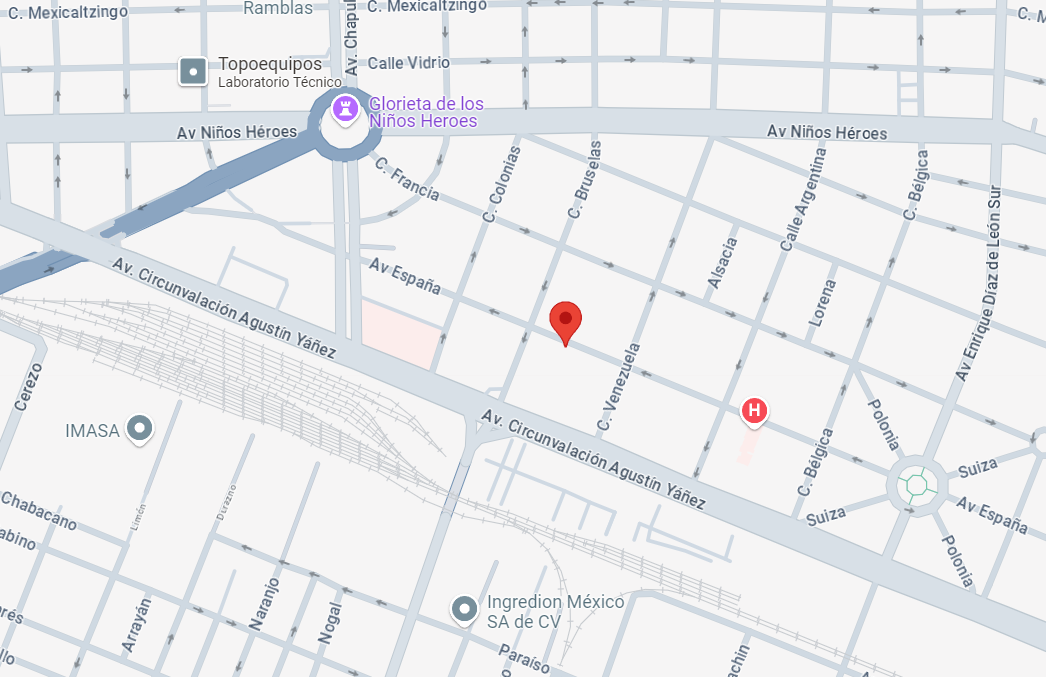
\includegraphics[width=0.8\textwidth]{Imagenes/ubicacion.png}
	\caption{Mapa ubicación Laboratoriso PiSA S.A DE C.V}\label{a1}
\end{figure}


% Poner la direcci�n y un mapa que puede salir de maps.google.com


\section{Misión}
Somos un Grupo de Empresas Responsables, confiables, éticas, con vocación de servicio; comprometidas con sus colaboradores y la salud.

\section{Visión}
Permanencia a través de innovación y crecimiento acelerado en México y en el extranjero.
	
\section{Organigrama}

\begin{figure}[H]
	\centering
	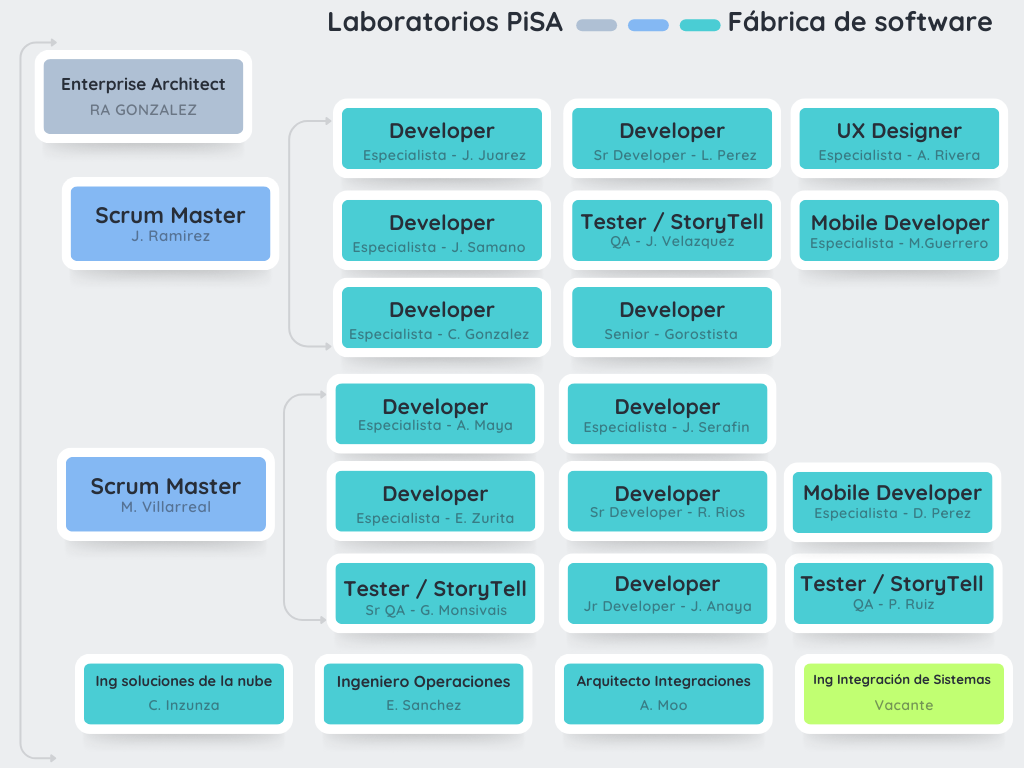
\includegraphics[width=0.9\textwidth]{Imagenes/OrganigramaPisa.png}
	\caption{Organigrama de Fábrica de Software}\label{a1}
\end{figure}
	
\section{Giro de la empresa}

PiSA Farmacéutica es una empresa dedicada a la fabricación, comercialización y distribución de medicamentos y dispositivos médicos en el tratamiento de un amplio ramo de la salud

\section{Historia}

PiSA Farmacéutica es una empresa mexicana, con 77 años de historia, desarrollando productos y servicios integrales para los segmentos de salud pública y privada en México, Estados Unidos, Latinoamérica y el Caribe.

\newpage
% -------------------------------- CAPITULO PROBLEM�TICA --------------------------------------
%____________________________________________________________________________________________________________________
	
\chapter{Problemática y Descripción del Proyecto}
\newpage

% En esta secci�n se deber� redactar un planteamiento de la problem�tica que se pretende resolver.
\section{Problemática}

	Path de Ayuda surge como una solución a la ausencia de un sistema visual de monitoreo en tiempo real en la planta de Formas Sólidas, lo que representa un desafío significativo en la gestión del proceso de fabricación.\\
	
	La falta de un sistema de monitoreo genera retrasos en la planificación de cambios y limpiezas debido a la carencia de información oportuna, lo que dificulta la disponibilidad de los formatos y piezas necesarias para garantizar la continuidad operativa.\\

	Asimismo, la ausencia de un mecanismo automatizado para la gestión de alertas afecta la capacidad de respuesta ante problemas técnicos o logísticos, prolongando los tiempos de resolución y afectando directamente la eficiencia y productividad de la planta.

%Escribir un resumen de su proyecto en donde se hable del aspecto económico, operativo, técnico, humano, objetivos, etc.
\section{Descripción del Proyecto}

	Path de Ayuda es un sistema diseñado para optimizar la gestión del proceso de fabricación mediante la visualización continua del estado de producción en cada una de las dieciséis líneas de acondicionado. Este sistema proporciona información en tiempo real sobre el avance de los lotes, garantizando una comunicación eficiente y una rápida capacidad de respuesta ante incidentes.\\
	
	Gracias a su implementación, el personal corporativo, gerencial y operativo podrá tomar decisiones oportunas para minimizar los tiempos de respuesta y mejorar la resolución de problemas.\\
	
	Contribuye significativamente a la eficiencia y productividad de la planta, reduciendo los tiempos de inactividad, optimizando la planificación de recursos y mejorando la trazabilidad de los procesos.


%Describir cual es el objetivo general que persigue el proyecto.
\subsection{Objetivo General}

	Realizar una documentación detallada para la implementación de un sistema de monitoreo en tiempo real, incluyendo la elaboración de pruebas de calidad. Además, se evaluarán propuestas de empresas para el desarrollo del sistema. La aplicación, denominada Path de Ayuda, estará enfocada en gestionar los requisitos operativos y de gestión, optimizando la planificación y la toma de decisiones en el proceso de fabricación.


%Describir cuales son los objetivos específicos que persigue el proyecto. Mínimo deben ser dos y estos deben abonar al objetivo general
\subsection{Objetivos Específicos}

	1. Documentar las necesidades operativas y funcionales del sistema de monitoreo, asegurando la participación de los stakeholders clave para definir los requisitos.\\
	
	2. Establecer los requisitos funcionales y no funcionales de la aplicación Path de Ayuda, incluyendo funcionalidades como visualización de líneas de producción y gestión de alertas.\\
	
	3. Crear escenarios y casos de prueba para evaluar la viabilidad del sistema, abarcando pruebas de integración, carga y usabilidad.\\
	
	4. Ejecutar pruebas unitarias, de integración y de aceptación para asegurar que el sistema cumpla con los estándares de rendimiento, seguridad y funcionalidad.\\
	
	5. Solicitar y analizar propuestas de empresas para seleccionar la opción más adecuada según criterios técnicos, económicos y operativos.\\
	
	6. Validar el funcionamiento y rendimiento del sistema mediante pruebas de carga, estrés y funcionalidad para garantizar su efectividad antes de la implementación.. 
	
	
%Describir de manera detallada las actividades para el desarrollo de la estadía y/o proyecto (Diagrama de Gantt).
\subsection{Planeación}



%CAPITULO MARCO TEÓRICO: bases teorícas del proyecto. conceptos básicos y antecedentes o información existente.
%____________________________________________________________________________________________________________________
	
\chapter{Marco Teórico}
\newpage


\section{MongoDB}
	
	Como lo dijo \citeauthor{ArBre}, \citeyear  Acelere la innovación a escala, aborde las necesidades de datos de cualquier aplicación rápidamente, acelere el tiempo de obtención de valor y reduzca la complejidad seleccionando y eligiendo lo que necesita de una colección integrada de servicios de infraestructura de datos y bases de datos.  \cite{mongodb} es un formato válido, pero no es APA que solicitan en la memoria,  para cumplir con la norma podemos hacer la referencia de esta manera (\citeauthor{mongodb}, \citeyear{mongodb}) y en (\citeauthor{ArBre}, \citeyear{ArBre})
	

%CAPITULO DESARROLLO DEL PROYECTO: procedimiento o descripci�n de las actividades realizadas, como es un desarrollo es importante
%____________________________________________________________________________________________________________________


\chapter{Desarrollo del Proyecto}
\newpage
	
\section{Requerimientos}
	
\section{Análisis y Diseño}

\section{Implementación}

\section{Pruebas}


% CAPITULO RESULTADOS(estatus del proyecto y posibles mejoras) Y CONCLUSIONES(problemas presentados, costos, restrasos, cumplimiento de objetivos, etc)
%____________________________________________________________________________________________________________________
	
	
\chapter{Resultados y Conclusiones}
\newpage
	
\section{Resultados}

\section{Conclusiones}


% -------------------------- ANEXOS
%____________________________________________________________________________________________________________________
	

\newpage
% APENDICE O ANEXO (infoemacion adicional que se quiera anexar o agregar
% BIBLIOGRAFIA
\appendix
	
%\chapter{Bibliograf\check{}�a}
%\bibliographystyle{apalike}
\bibliographystyle{unsrtnat}
	
	
\begin{itemize}
	\item A
	\item B
	\item C
\end{itemize}

	
\bibliography{biblio}

\newpage	
\chapter{Glosario}

\begin{description}
	\item[Asesor Acadámico] Persona encargada de regañar a los alumnos
\end{description}
	
%Otro apendice

\end{document} 
